
\chapter{Analyse et spécification des besoins}
\label{chap:Analyse et spécification des besoins}

Ce chapitre présente l'analyse de l'existant et la spécification des besoins pour l'intégration de Bancontact by Payconiq. Nous examinerons les méthodes de paiement actuelles, les spécificités du marché belge, l'architecture existante, ainsi que les besoins fonctionnels et non fonctionnels.
\pagebreak

\section{Étude de l’existant}
\subsection{Méthodes de paiement actuelles}
Le site e-commerce de la marque propose actuellement une gamme diversifiée de méthodes de paiement reconnues mondialement, comprenant :
\begin{itemize}
    \item Visa
    \item MasterCard
    \item PayPal
    \item Klarna Pay Now
    \item Klarna Pay Later
    \item Chanel Gift Card
\end{itemize}
Bien que ces options répondent efficacement aux besoins d'une clientèle internationale, elles ne tiennent pas compte des spécificités locales de certains marchés clés, en particulier celui de la Belgique.
\subsection{Particularités du marché belge}
En Belgique, Bancontact s'est imposé comme l'une des méthodes de paiement privilégiées. Initialement conçu comme un système de paiement par carte de débit national, Bancontact est devenu un élément incontournable du paysage financier belge. Cette solution offre aux consommateurs belges la possibilité d'effectuer des paiements directs depuis leur compte bancaire, que ce soit en magasin, en ligne ou via une application mobile.
Face à l'évolution rapide des technologies et des attentes des consommateurs, Bancontact a réalisé une fusion stratégique avec Payconiq, une solution de paiement mobile innovante. Cette alliance a donné naissance à Bancontact by Payconiq, offrant aux utilisateurs belges une solution de paiement intégrée couvrant à la fois les transactions par carte et les paiements mobiles via une application dédiée.
L'adoption massive de cette solution en Belgique en fait un élément incontournable pour tout e-commerce aspirant à s'implanter solidement sur ce marché. Les chiffres parlent d'eux-mêmes : en 2023, près de 2 millions de Belges ont utilisé Payconiq pour leurs paiements mobiles, soulignant l'importance cruciale de cette méthode dans l'écosystème des paiements locaux.
\subsection{Justification de l'intégration de Bancontact by Payconiq}
L'intégration de Bancontact by Payconiq sur notre plateforme e-commerce présente plusieurs avantages stratégiques majeurs, particulièrement pour conquérir et fidéliser la clientèle belge :
\begin{itemize}
    \item [$\bullet$]\textbf{Adoption généralisée :} Avec une base d'environ 2 millions d'utilisateurs Payconiq et une forte pénétration de Bancontact dans les habitudes de paiement quotidiennes, cette solution est profondément ancrée dans le comportement des consommateurs belges.
    \item [$\bullet$]\textbf{Simplicité et ergonomie :} L'application "Payconiq by Bancontact" offre une expérience de paiement fluide et intuitive, reposant sur un simple scan de QR code, ce qui optimise considérablement le parcours client.
    \item [$\bullet$]\textbf{Sécurité renforcée :} La synergie entre les systèmes Bancontact et Payconiq garantit un niveau de sécurité optimal pour les transactions, s'appuyant sur des protocoles de sécurité robustes et éprouvés.
    \item [$\bullet$]\textbf{Interopérabilité bancaire :} Le support étendu de Payconiq par les principales institutions bancaires belges facilite son adoption et renforce la commodité pour les clients, en centralisant leurs opérations financières.
    \item [$\bullet$]\textbf{Essor des paiements mobiles :} Face à la croissance exponentielle des paiements mobiles en Belgique, l'intégration de solutions comme Payconiq s'avère cruciale pour capter et fidéliser une clientèle, particulièrement auprès des jeunes générations habituées aux transactions via smartphone.
\end{itemize}
\subsection{Architecture du processus de paiement actuel}
Le processus de paiement en place repose sur l'interaction harmonieuse de plusieurs systèmes interdépendants, chacun jouant un rôle déterminant dans la sécurisation des transactions et l'optimisation du traitement des commandes. Les composants clés du système sont les suivants :
\begin{itemize}
    \item [$\bullet$]\textbf{Hybris :} Plateforme e-commerce centrale, Hybris est responsable de la création des commandes une fois le paiement validé. Après la soumission d'une commande par l'utilisateur, Hybris communique avec Adyen pour le traitement du paiement. Une fois la confirmation reçue, Hybris crée officiellement la commande et notifie Fluent pour la gestion de l'expédition et du suivi.
    \item [$\bullet$]\textbf{Adyen :} En tant que fournisseur de services de paiement, Adyen gère la transaction financière. Il traite les détails du paiement transmis par Hybris, réalisant des actions telles que l'autorisation, la capture des fonds, ou la gestion des abonnements. Adyen joue un rôle clé dans la sécurisation et la validation des paiements avant la finalisation de la commande.
    \item [$\bullet$]\textbf{Fluent :} Système de gestion logistique, Fluent est responsable du cycle de vie de la commande après sa création dans Hybris. Il assure le suivi du processus de traitement, y compris la préparation de l'expédition, et met à jour les statuts de la commande (par exemple, "CREATED", "PENDING PAYMENT", "CANCELLED"). Fluent communique également avec Hybris pour informer les utilisateurs de l'état de leur commande.
\end{itemize}
Pour mieux comprendre le fonctionnement de ces composants, examinons le flux du processus de paiement étape par étape :
\begin{enumerate}
    \item \textbf{Initiation :} Le client valide son panier et soumet sa commande.
    \item \textbf{Transmission :} Hybris communique les informations de paiement à Adyen.
    \item \textbf{Traitement :} Adyen exécute la transaction et renvoie une confirmation à Hybris.
    \item \textbf{Création :} Hybris enregistre la commande et notifie Fluent pour la gestion logistique.
    \item \textbf{Suivi :} Fluent assure la gestion des statuts de commande et informe Hybris pour la mise à jour du client.
\end{enumerate}
\section{Etude fonctionnelle et non fonctionnelle}

Dans le cadre de l'intégration de Payconiq à la plateforme e-commerce du client, il est essentiel de définir clairement les besoins fonctionnels et non fonctionnels du projet. 
Cette étude permettra d'identifier les exigences spécifiques liées à cette intégration, assurant ainsi une mise en œuvre réussie et une expérience utilisateur optimale. 
\subsection{Exigences fonctionnelles}

\subsubsection{Identification des fonctionnalités}


\subsubsection{Diagramme de cas d’utilisation}

Les diagrammes des cas d'utilisation décrivent les fonctions générales et la portée d'un système. Ces diagrammes identifient également les interactions entre le système et ses acteurs.

Nous synthétisons dans ce paragraphe tout ce qui a été dit dans la phase d’analyse. Nous présentons le diagramme de cas d’utilisation de notre application et introduisons les cas d’utilisation qui la composent.

\begin{figure}[H]
    \centering
    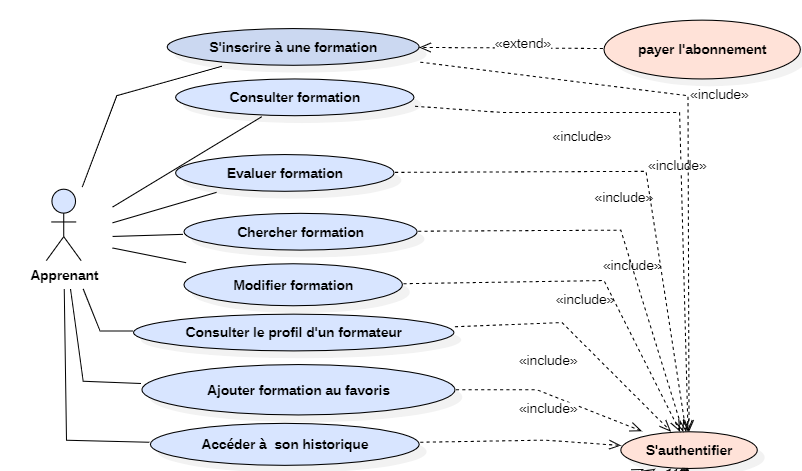
\includegraphics[width=15cm]{Figures/apprenant.PNG}
    \caption{Diagramme de cas d’utilisation d'apprenant}
\end{figure}

\subsubsection{Description textuelle de cas d’utilisation}

\begin{minipage}{\textwidth}
\begin{table}[H]
\centering
\begin{tabular}{| m{8cm} | m{8cm} |}
\hline
\multicolumn{2}{|c|}{\textbf{UC 1:} Payer l'abonnement d'une formation} \\ \hline
\textbf{Acteurs} & Apprenant \\ \hline
\textbf{But} & Permettre à un apprenant d'accéder à une formation disponible sur la plateforme et voir les vidéos \\ \hline
\textbf{Préconditions} & \textbf{Postconditions} \\ \hline
- S'authentifier. & - Voir les vidéos \\ \hline
\textbf{Scénario Principal} & \textbf{Scénario Alternatif} \\ \hline
\begin{enumerate}
    \item S'authentifier.
    \item Naviguer vers la page de la formation.
    \item Choisir la formation.
    \item Cliquer sur "S'inscrire".
    \item Effectuer le paiement.
    \item vérifier si le paiement est autorisé.
    \item Redirection vers la page de confirmation de paiement.
\end{enumerate} & 
\begin{enumerate}
    \item S'authentifier.
    \item Naviguer vers la page de la formation.
    \item Choisir la formation.
    \item Cliquer sur "S'inscrire".
    \item Effectuer le paiement.
    \item vérifier si le paiement est autorisé.
    \item Redirection vers la page d’erreur.
\end{enumerate} \\ \hline
\end{tabular}
\caption{Description Textuelle du Cas d'Utilisation "Payer l'abonnement d'une formation"}
\label{tab:use_case_description_1}
\end{table}
\end{minipage}

\newpage

\begin{minipage}{\textwidth}
\begin{table}[H]
\centering
\begin{tabular}{| m{8cm} | m{8cm} |}
\hline
\multicolumn{2}{|c|}{\textbf{UC 2:} Ajouter une formation} \\ \hline
\textbf{Acteurs} & Administrateur \\ \hline
\textbf{But} & Permettre à un administrateur d'ajouter une formation à la plateforme avec ses chapitres et ses vidéos \\ \hline
\textbf{Préconditions} & \textbf{Postconditions} \\ \hline
- S'authentifier. & Formation ajoutée \\ \hline
\textbf{Scénario Principal} & \textbf{Scénario Alternatif} \\ \hline
\begin{enumerate}
    \item S'authentifier.
    \item Naviguer vers la page d'ajout de formation.
    \item Remplir les informations nécessaires pour la formation.
    \item Ajouter les chapitres.
    \item Ajouter les vidéos.
    \item Cliquer sur le bouton "Enregistrer".
    \item Un message de confirmation est affiché.
\end{enumerate} & 
\begin{enumerate}
    \item S'authentifier.
    \item Naviguer vers la page d'ajout de formation.
    \item Remplir les informations nécessaires pour la formation.
    \item Ajouter les chapitres.
    \item Ajouter les vidéos.
    \item Cliquer sur le bouton "Enregistrer".
    \item Un message d'erreur spécifiant les champs incorrects ou manquants est affiché.
\end{enumerate} \\ \hline
\end{tabular}
\caption{Description Textuelle du Cas d'Utilisation "Ajouter une formation"}
\label{tab:use_case_description_2}
\end{table}
\end{minipage}





\subsubsection{Diagramme de séquence de système}

\subsubsection*{Diagramme de séquence de l’authentification}

L’authentification est l’étape primordiale pour toutes les fonctionnalités. L'interaction débute par l’utilisateur qui saisit ses informations d'authentification (username et mot de passe) et les envoie au système.
Dans le premier cas, le système transmet ces informations à sa base de données pour vérification. Si les informations sont correctes, le système redirige l'utilisateur vers la page d'accueil.
Dans le deuxième cas, si les informations d'authentification sont incorrectes, la base de données envoie une réponse négative au système. Le système informe alors l'utilisateur que les informations saisies sont incorrectes, et il est redirigé vers la page d'authentification pour qu'il puisse réessayer.


\begin{figure}[H]
    \centering
    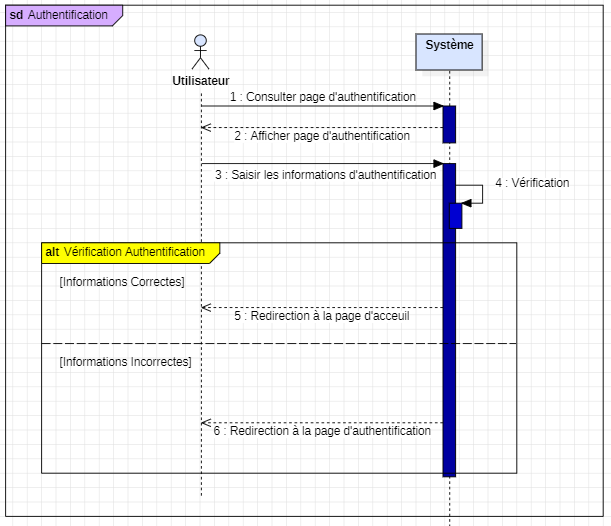
\includegraphics[width=19cm]{Figures/diagrammeDeSequenceAuthentification.png}
    \caption{Diagramme De Séquence De l'Authentification}
\end{figure}

\subsubsection*{Diagramme de séquence d’ajouter une formation}

Ce diagramme montre comment un administrateur ajoute une formation. L'administrateur clique sur "ajouter formation", un formulaire s'affiche, et les informations sont saisies. Le processus se poursuit avec l'ajout de chapitres et de vidéos, l'importation des vidéos et l'envoi des données pour la création de la formation. Une notification est affichée pour indiquer si la création a réussi ou échoué.

\begin{figure}[H]
    \centering
    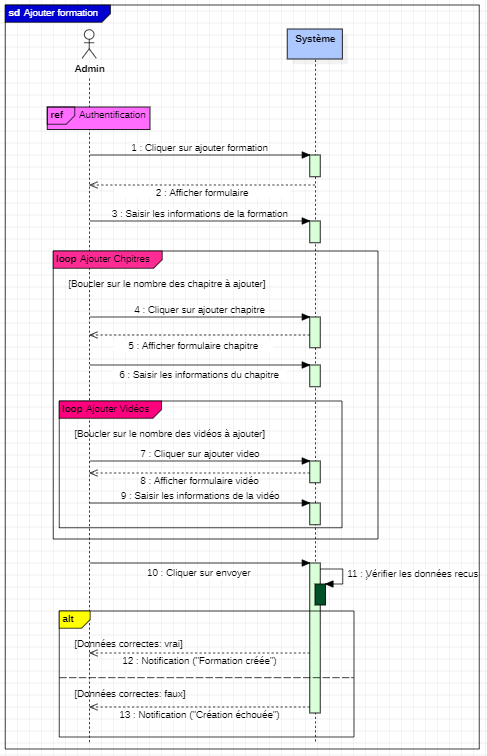
\includegraphics[width=15cm]{Figures/diagrammeDeSequenceCreerCourse.PNG}
    \caption{Diagramme De Séquence d'Ajouter Une Formation}
\end{figure}

\subsubsection*{Diagramme de séquence d'ajouter un formateur}

Le diagramme de séquence montre le processus par lequel un administrateur ajoute un formateur. L'administrateur clique sur "ajouter formateur" et le système affiche un formulaire à remplir. Après la soumission du formulaire, le système envoie une requête à la base de données pour créer le formateur. Si la création réussit, le système notifie l'administrateur que le formateur a été ajouté avec succès. En cas d'échec, une notification d'échec est envoyée.

\begin{figure}[H]
    \centering
    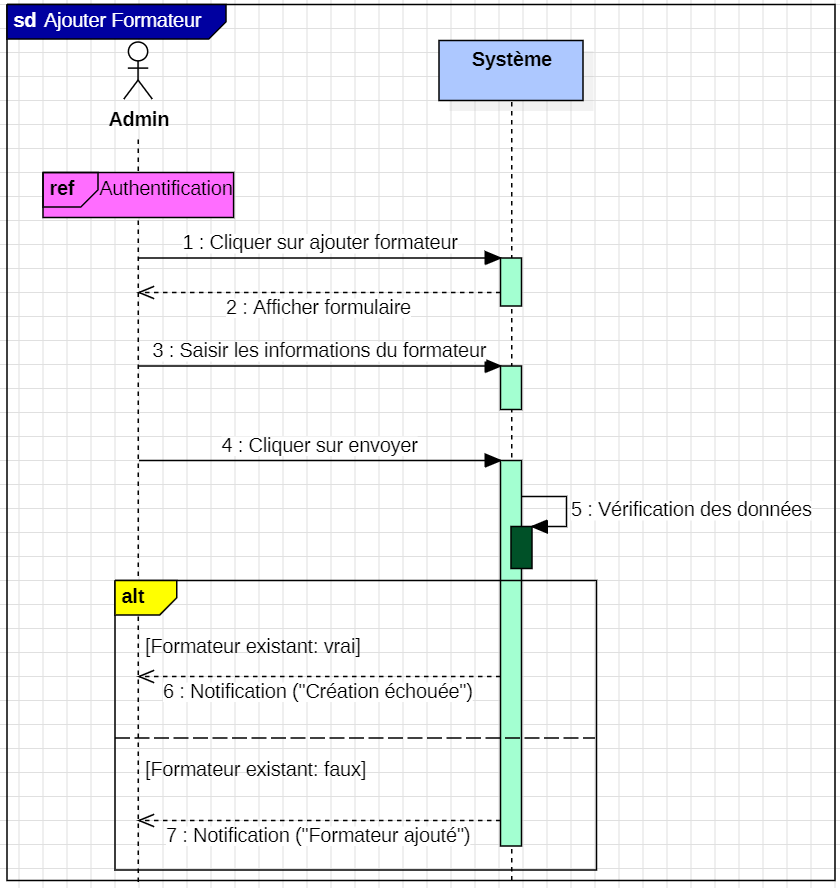
\includegraphics[width=17cm]{Figures/diagrammeDeSequenceAddAuthor.PNG}
    \caption{Diagramme De Séquence D'ajouter Formateur}
\end{figure}


\subsection{Exigences non-fonctionnelles}


Ce sont les besoins qui permettent d’améliorer la qualité des services de la plateforme comme la convivialité et l’ergonomie des interfaces et l’amélioration du temps de réponse. Parmi ces besoins, on cite :

\begin{itemize}
    \item[$\bullet$] \textbf{Convivialité:} La future application doit être facile à utiliser. En effet, les interfaces utilisateur doivent être conviviales c’est-à-dire simples, ergonomiques et adaptées à l’utilisateur.
    \item[$\bullet$] \textbf{Maintenabilité:} Toute architecture est exposée à des évolutions au niveau de la technologie d’implémentation. La solution doit avoir un grand niveau d’abstraction pour faciliter les nouvelles implémentations.
    \item[$\bullet$] \textbf{Performance:} Le temps de réponse doit être le plus court possible.
    \item[$\bullet$] \textbf{Disponibilité:} Lorsque n’importe quel utilisateur désire consulter la plateforme, elle doit être disponible.
    \item[$\bullet$] \textbf{Sécurité:} La plateforme doit protéger les données personnelles des utilisateurs, garantir l'intégrité des cours et du contenu.
\end{itemize}
\section*{Conclusion}
La phase d'analyse de l'existant et de spécification des besoins est cruciale pour le succès de notre projet. Nous avons abordé cette phase en examinant l'architecture actuelle, en identifiant les acteurs clés et les cas d'utilisation spécifiques au marché belge. Ensuite nous avons entamé l'analyse des besoins fonctionnels et non fonctionnels. Dans les chapitres suivants, nous aborderons la conception détaillée du projet d'intégration.